\hypertarget{polygon__holes_8h}{
\section{Referencia del Archivo polygon\_\-holes.h}
\label{polygon__holes_8h}\index{polygon_holes.h@{polygon\_\-holes.h}}
}


\subsection{Descripci\'{o}n detallada}
Declaraciones del Objeto Poligono con huecos 

Definici\'{o}n en el archivo \hyperlink{polygon__holes_8h-source}{polygon\_\-holes.h}.

{\tt \#include $<$stdbool.h$>$}\par
{\tt \#include \char`\"{}point.h\char`\"{}}\par
{\tt \#include \char`\"{}polygon.h\char`\"{}}\par


Dependencia gr\'{a}fica adjunta para polygon\_\-holes.h:\begin{figure}[H]
\begin{center}
\leavevmode
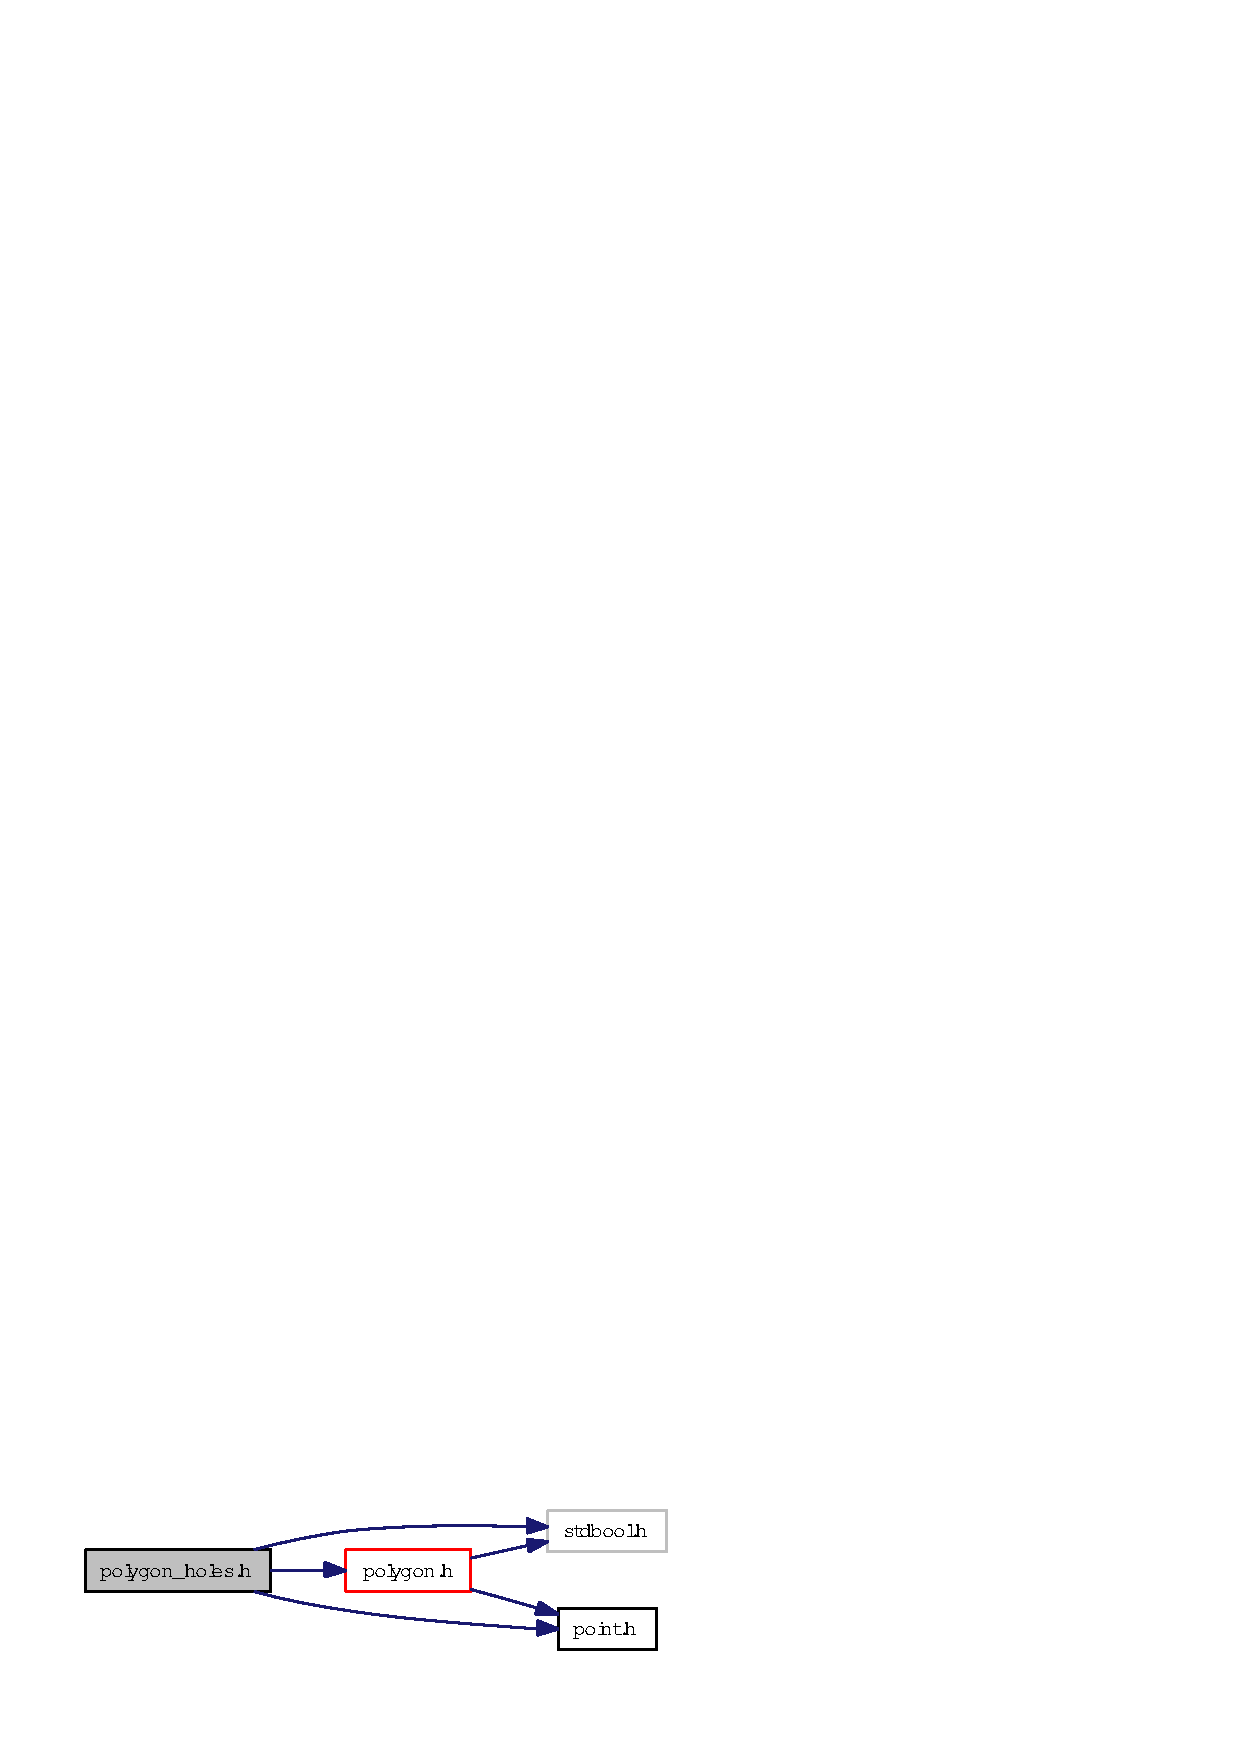
\includegraphics[width=162pt]{polygon__holes_8h__incl}
\end{center}
\end{figure}


Este gr\'{a}fico muestra que archivos directa o indirectamente incluyen a este archivo:\begin{figure}[H]
\begin{center}
\leavevmode
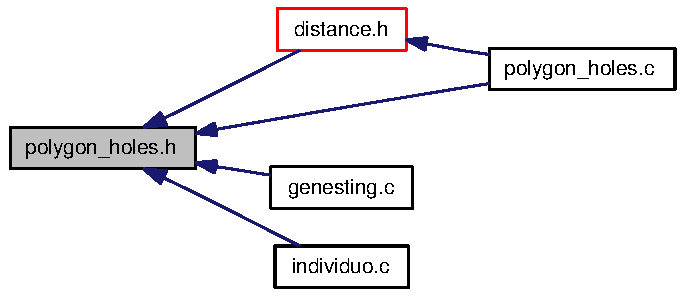
\includegraphics[width=182pt]{polygon__holes_8h__dep__incl}
\end{center}
\end{figure}
\subsection*{Clases}
\begin{CompactItemize}
\item 
struct \hyperlink{struct__polygon__holes}{\_\-polygon\_\-holes}
\end{CompactItemize}
\subsection*{Tipos definidos}
\begin{CompactItemize}
\item 
typedef \hyperlink{struct__polygon__holes}{\_\-polygon\_\-holes} \hyperlink{group__geometry_g1137695e6ed0a9b25685f8bf3ccdb45f_g1137695e6ed0a9b25685f8bf3ccdb45f}{polygon\_\-holes}
\end{CompactItemize}
\subsection*{Funciones}
\begin{CompactItemize}
\item 
float \hyperlink{group__geometry_g380cdcfa6caf51828c8d06f4518a4084_g380cdcfa6caf51828c8d06f4518a4084}{polygonholes\_\-area} (\hyperlink{struct__polygon__holes}{polygon\_\-holes} $\ast$p)
\item 
float \hyperlink{group__geometry_g7cf8b3f8c76179bb936754bbbf510999_g7cf8b3f8c76179bb936754bbbf510999}{polygonholes\_\-volumen} (\hyperlink{struct__polygon__holes}{polygon\_\-holes} $\ast$p)
\item 
bool \hyperlink{group__geometry_g35a6dd45f6d0cbed26ef8a69ed34a2e9_g35a6dd45f6d0cbed26ef8a69ed34a2e9}{polygonholes\_\-pointin} (\hyperlink{struct__polygon__holes}{polygon\_\-holes} $\ast$p, \hyperlink{struct__point}{point} $\ast$f)
\item 
bool \hyperlink{group__geometry_g496bae87588cb5710ced80f713da98ad_g496bae87588cb5710ced80f713da98ad}{polygonholes\_\-polygonin} (\hyperlink{struct__polygon__holes}{polygon\_\-holes} $\ast$p, \hyperlink{struct__polygon}{polygon} $\ast$q)
\item 
bool \hyperlink{group__geometry_g139317720b027c782db9424256ba2c2d_g139317720b027c782db9424256ba2c2d}{polygonholes\_\-pointinhole} (\hyperlink{struct__polygon__holes}{polygon\_\-holes} $\ast$p, \hyperlink{struct__point}{point} $\ast$f)
\end{CompactItemize}
